\section{Architecture globale}
    \label{sec:archiGlobale}
    
    Afin de mieux fixer les idées quant aux fonctionnalités de Glasir, voici une présentation de son utilisation et de son interface.
	    
    \subsection{Diagramme de cas d'utilisation}
    \label{sec:casutil}
    
    L'utilisateur-type de notre outil d'analyse serait un expert en sécurité connaissant déjà le formalisme des ADTrees. C'est donc l'acteur qui a été choisi pour le diagramme de cas d'utilisation de la {\sc Figure}~\ref{fig:use_case}, qui représente l'ensemble des actions possibles à partir de Glasir. Afin de mieux comprendre ce diagramme, un petit rappel sur le formalisme UML s'impose. En effet, si l'on prend deux évènements A et B, les termes \og étendre \fg{} et \og inclure \fg{} associés aux flèches ont une signification bien particulière :

    \begin{itemize}
    \item[] $ A \stackrel{\text{\og inclure \fg{}}}{\longrightarrow} B$ signifie que si $A$ est réalisé, $B$ l'est {\bf forcément} ;
    \item[] $ B \stackrel{\text{\og étendre \fg{}}}{\longrightarrow} A$ signifie que si $A$ est réalisé, $B$ {\bf peut} l'être mais pas obligatoirement.
    \end{itemize}

    \begin{figure}[H]
        \centering
        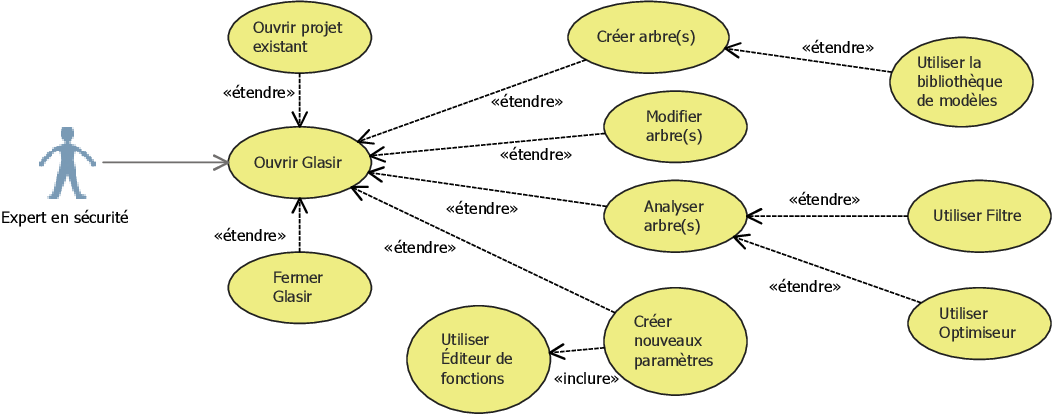
\includegraphics[height=0.5\textwidth]{figure/UseCaseDiagram.png}
        \caption{Diagramme de cas d'utilisation de Glasir.}
        \label{fig:use_case}
    \end{figure}

    Les fonctionnalités de Glasir apparaissent donc maintenant clairement. Grâce à cet outil, l'utilisateur pourra effectuer les actions suivantes : 

    \begin{itemize}
    \item charger un projet sauvegardé ;
    \item créer de nouveaux ADTrees, en utilisant ou non la bibliothèque de modèles ;
    \item modifier des ADTrees déjà existants ;
    \item analyser les ADTrees du projet en cours, à l'aide du Filtre ou de l'Optimiseur ;
    \item créer de nouveaux paramètres pour ADTool par le biais de l'Éditeur de fonctions.
    \end{itemize}  

    Toutes ces possibilités seront accessibles facilement grâce à une interface utilisateur claire et fonctionnelle, dont un prototype est présenté dans la {\sc Section}~\ref{sec:interface}.      
    
    \subsection{Prototype d'interface}
    \label{sec:interface}
    
    La {\sc Figure}~\ref{fig:interface} représente un prototype d'interface pour Glasir. Ce prototype n'est pas définitif, mais permet de donner un avant-goût de l'organisation générale du programme. 

    \begin{figure}[h!]
        \centering
        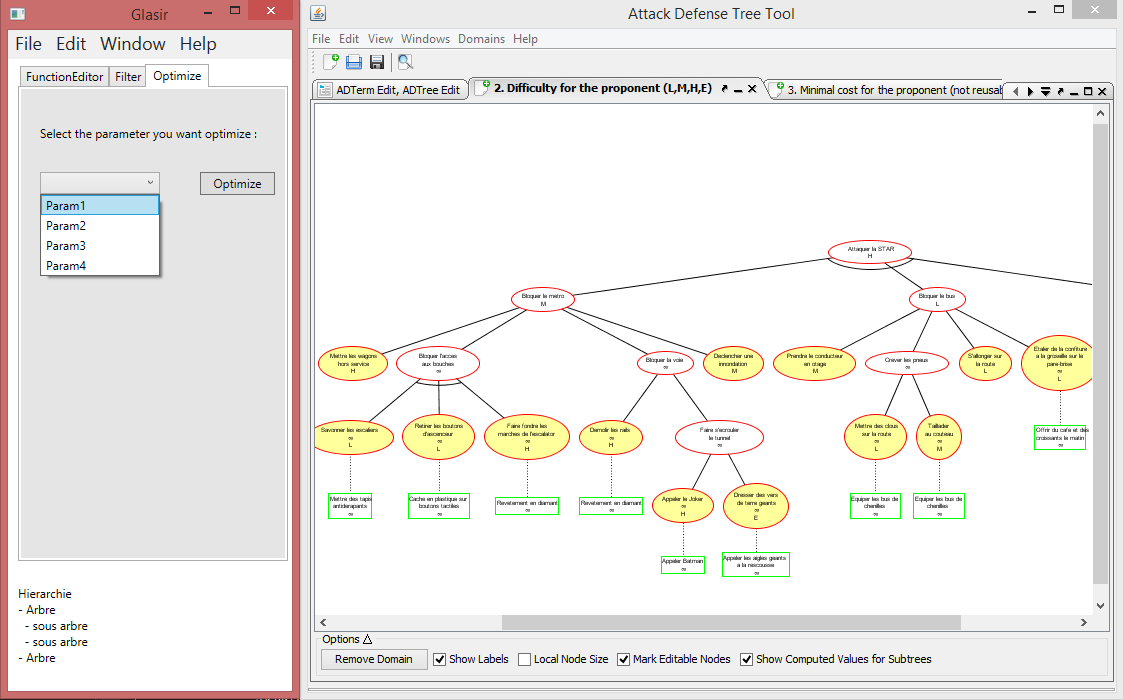
\includegraphics[height=0.72\textwidth]{figure/interface.png}
        \caption{Prototype de l'interface de Glasir.}
        \label{fig:interface}
    \end{figure}
    
    \begin{figure}[h!]
        \centering
        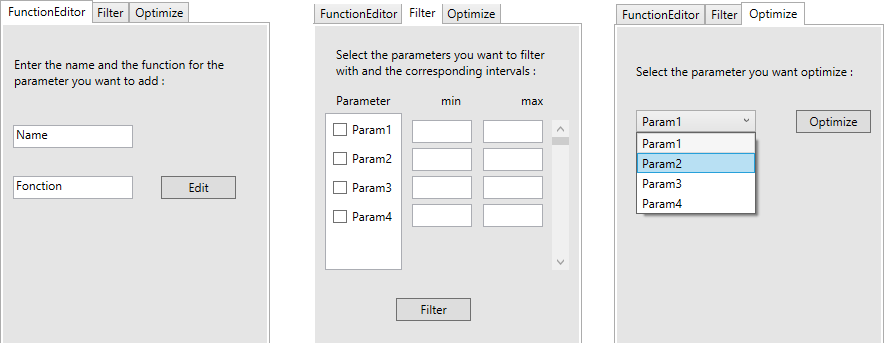
\includegraphics[height=0.42\textwidth]{figure/ongletsGlasir.png}
        \caption{Prototype des panneaux permettant d'utiliser les fonctionnalités de Glasir.}
        \label{fig:panneaux}
    \end{figure}
    
L'interface de Glasir est scindée en deux parties distinctes : la fenêtre de Glasir à proprement parler (située à gauche sur le prototype de la {\sc Figure}~\ref{fig:interface}), et les fenêtres des instances d'ADTool (situées à droite). Au sein de la fenêtre de Glasir, les fonctionnalités du Filtre, de l'Optimiseur et de l'Éditeur de fonctions sont accessibles facilement. La barre de menu (située en haut à gauche sur le prototype de la {\sc Figure}~\ref{fig:interface}) permet de créer un nouveau projet, d'en charger un déjà existant, ou encore de sauvegarder le projet courant.
    
    La {\sc Figure}~\ref{fig:panneaux} illustre également un prototype des panneaux qui permettent d'accéder aux fonctionnalités principales de Glasir. Ces fonctionnalités sont détaillées dans les {\sc Sections}~\ref{sec:diagClass} et \ref{sec:modules}.  